% ----------------------------------------------------
\begin{frame}
  \titlepage
\end{frame}
% ----------------------------------------------------
\note{Recordar brevemente lo visto: el modelo de negociación (sesión 3) y la política doméstica, democracia, alianzas y seguridad colectiva (sesión 4). Hoy: violencia por actores no estatales -- guerras civiles y terrorismo. Es el tipo de conflicto más frecuente en el mundo actual.}

% ----------------------------------------------------
\begin{frame}
\frametitle{Hoy}
\centering
\vspace{1.5em}
\begin{itemize}
  \setlength{\itemsep}{10pt}
  \item Guerras civiles: ¿por qué ocurren y por qué duran?
  \item Insurgencia y contrainsurgencia
  \item Terrorismo: lógica y estrategias
  \item Respuestas al terrorismo
\end{itemize}
\end{frame}
% ----------------------------------------------------
\note{}

% ====================================================
\section{Violencia por actores no estatales}
% ====================================================

% ----------------------------------------------------
\begin{frame}[plain]
  \begin{tikzpicture}[remember picture, overlay]
    \node[at = (current page.center), yshift = 0cm] (cover) {%
      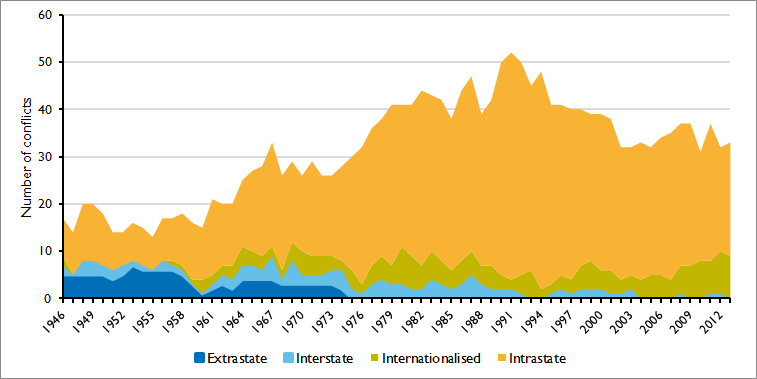
\includegraphics[keepaspectratio, height=\paperheight]{../img/armed_conflicts.png}};
  \end{tikzpicture}
\end{frame}
% ----------------------------------------------------
\note{Gráfico de conflictos armados en el mundo. Desde el fin de la Guerra Fría, la inmensa mayoría de los conflictos armados son \textit{intraestatales} (guerras civiles), no interestatales. Éste es el tipo de violencia política más común hoy.}

% ----------------------------------------------------
\imageframe{../img/9-11}
\note{el 11s como catalisto}
% ----------------------------------------------------


% ----------------------------------------------------
\begin{frame}
\frametitle{El panorama actual}
\centering

\begin{itemize}
  \item Las guerras interestatales han disminuido
  \item Pero las \textbf{guerras civiles} son el tipo de conflicto dominante
  \item<2-> Actores: gobiernos y grupos armados no estatales (rebeldes, guerrillas, milicias, organizaciones terroristas...)
  \item<2-> Las herramientas del modelo de negociación siguen siendo útiles
\end{itemize}

\end{frame}
% ----------------------------------------------------
\note{La violencia por actores no estatales es un tema de RRII, no solo de política doméstica, por varias razones:
\begin{itemize}
  \item Estados extranjeros a menudo apoyan a los combatientes (guerras proxy)
  \item Las guerras civiles generan refugiados, inestabilidad regional, contagio
  \item Las organizaciones internacionales (ONU) intervienen para mediar y mantener la paz
  \item Los grupos terroristas operan a nivel transnacional
\end{itemize}
Las mismas herramientas analíticas (intereses, información incompleta, problemas de compromiso, bienes indivisibles) se aplican.}


% ====================================================
\section{Definiciones}
% ====================================================

% ----------------------------------------------------
\begin{transitionframe}
Qué es cada cosa
\end{transitionframe}
\note{}
% ----------------------------------------------------

% ----------------------------------------------------
\begin{frame}
\frametitle{¿Qué es una guerra civil?}
\centering

\begin{itemize}
  \item Conflicto armado entre grupos \textbf{dentro} de un Estado
  \begin{itemize}
    \item Todos los actores en conflict estaban bajo la misma polity, y luchan por la soberanía política
    \item<2-> Gobierno vs.~rebeldes (lo más común)
    \item<2-> Varios grupos disputando el control (Estado colapsado, aunque generalmente uno es el incumbente)
  \end{itemize}
  \item<3-> Umbral de severidad (1.000 muertes en combate)
  \begin{itemize}
      \item La línea entre lo que es una guerra civil y simplemente un ataque o inestabilidad es más fina
  \end{itemize}
  \item<3-> La guerra civil es un \textit{tipo de conflicto}, el terrorismo es una \textit{estrategia}
\end{itemize}

\end{frame}
% ----------------------------------------------------
\note{Definición. La guerra civil y el terrorismo están relacionados pero son conceptos diferentes:
\begin{itemize}
  \item Guerra civil: se define por los \textit{actores} (grupos armados dentro de un Estado)
  \item Terrorismo: se define por las \textit{víctimas} (civiles) y los objetivos (políticos)
\end{itemize}
Los rebeldes a menudo usan tácticas terroristas, y los grupos terroristas a veces escalan su violencia hasta convertirse en insurgencias. Ejemplo: el Estado Islámico empezó como grupo terrorista y llegó a controlar un territorio del tamaño de Gran Bretaña.}

% ----------------------------------------------------
\begin{frame}
\frametitle{Tipos: tecnologías de la rebelión}
\centering

\begin{itemize}
  \item Guerras irregulares
  \begin{itemize}
    \item[] $\approx$ 34\% (1944--2004)
    \item[] (e.g. Nepal, Peru, etc)
  \end{itemize}
  \item Guerras convencionales
  \begin{itemize}
    \item[] $\approx$ 54\%
    \item[] (e.g. US, Spain, Sri Lanka, Syria)
  \end{itemize}
  \item Guerras simétricas, no-convencionales
  \begin{itemize}
    \item[] $\approx$ 12\%
    \item[] (Somalia, CAR)
  \end{itemize}
\end{itemize}

\end{frame}
\note{}
% ----------------------------------------------------

% ----------------------------------------------------
\begin{frame}
\frametitle{Tipos: otras dimensiones}
\centering

\begin{itemize}
  \item Étnicas vs no-étnicas
  \item Separatistas vs no separatistas 
  \begin{itemize}
    \item[] (A veces: `territoriales', `gubernamentales')
  \end{itemize}
  \item Internacionalizadas vs no internacionalizadas
  \item Otras: guerras revolucionarias, guerras vs conflictos baja intensidad...
\end{itemize}

\end{frame}
\note{}
% ----------------------------------------------------

% ----------------------------------------------------
\begin{frame}
\frametitle{¿Qué \textbf{no} es una guerra civil?}
\centering

\begin{itemize}
\setbeamercovered{transparent}
  \item<1> \textit{No} es violencia contra civiles
  \begin{itemize}
    \item Guerra $\neq$ violencia
  \end{itemize}
  \item<2> \textit{No} es terrorismo
  \begin{itemize}
    \item Aunque el terrorismo puede utilizarse dentro de las guerras
  \end{itemize}
  \item<3> \textit{No} es genocidio
  \begin{itemize}
    \item Cualquier guerra implica violencia de combate sostenida y bidireccional
  \end{itemize}
  \item<4> \textit{No} es violencia no estatal (p. ej., disturbios comunales)
  \begin{itemize}
    \item El Estado/gobierno es siempre uno de los participantes
  \end{itemize}
  \item<5> \textit{No} es un conflicto étnico
  \begin{itemize}
    \item Aunque existen guerras civiles \textit{étnicas} (pero el conflicto étnico también incluye disturbios étnicos o violencia étnica contra civiles)
  \end{itemize}
\end{itemize}

\end{frame}
\note{}
% ----------------------------------------------------

% ----------------------------------------------------
\begin{frame}<1-2>[label=vio_civ]
\frametitle{¿Qué es el terrorismo?}
\centering

\visible<2->{
\begin{itemize}
  \item ¿Violencia contra civiles?
\end{itemize}
}

\vspace{20pt}

\visible<3>{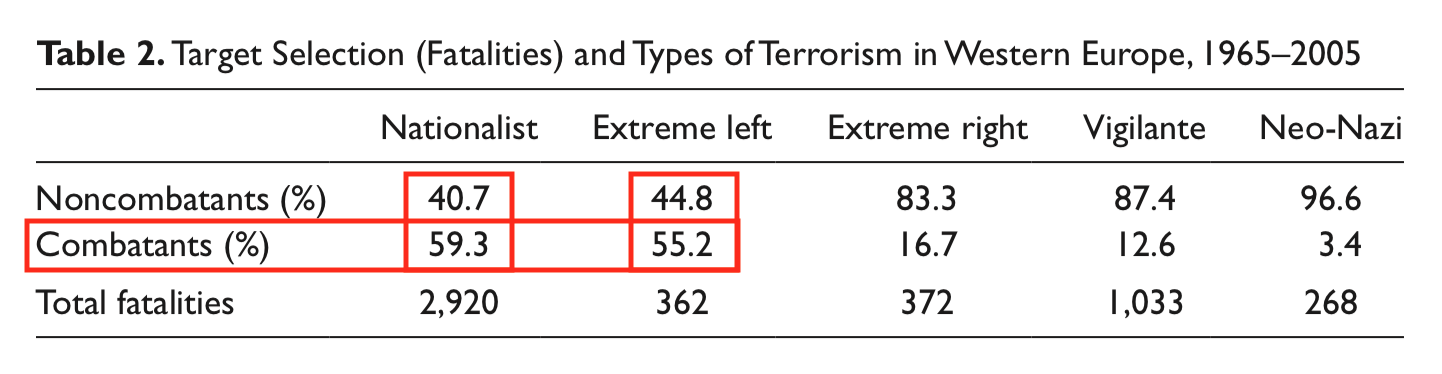
\includegraphics[width = \textwidth]{../img/combatants-noncombatant1}}
\visible<4>{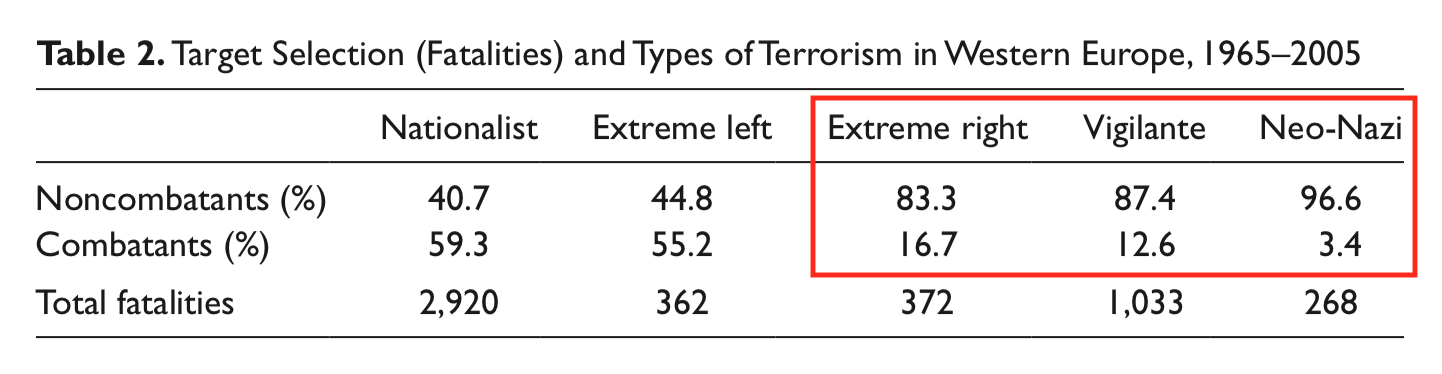
\includegraphics[width = \textwidth]{../img/combatants-noncombatant2}}

\end{frame}
% ----------------------------------------------------
\note{}

% ----------------------------------------------------
\begin{frame}
\frametitle{¿Violencia contra civiles?}
\centering

% ----------------------------------------------------
\begin{minipage}{.49\textwidth}\centering
  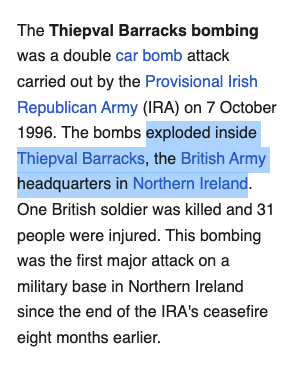
\includegraphics[width = \textwidth]{../img/thiepval_wiki1}
\end{minipage}\hfill
% ----------------------------------------------------
\begin{minipage}{.49\textwidth}\centering
  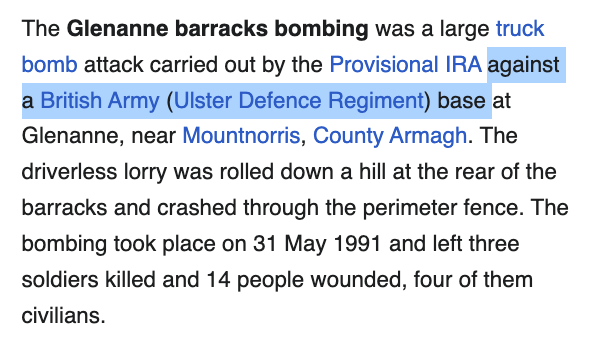
\includegraphics[width = \textwidth]{../img/glenanne_wiki}\\
  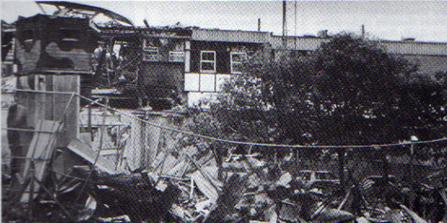
\includegraphics[width = \textwidth]{../img/glenanne}\\
\end{minipage}
% ----------------------------------------------------

\end{frame}
\note{}
% ----------------------------------------------------

\againframe<3->{vio_civ}
\note{}

% ----------------------------------------------------
\begin{frame}
\frametitle{¿Qué es el terrorismo?}
\centering

\begin{itemize}
  \item ¿Violencia ``comunicativa''?
\end{itemize}

\vspace{20pt}

\visible<2>{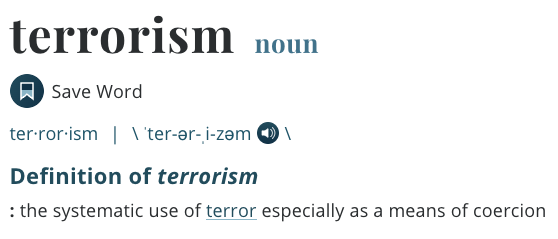
\includegraphics[width = 0.7\textwidth]{../img/webster}}

\end{frame}
\note{}
% ----------------------------------------------------

% ----------------------------------------------------
\imageframe{../img/wikipedia}
\note{}
% ----------------------------------------------------

% ----------------------------------------------------
\imageframe{../img/represion-franquista}
\note{}
% ----------------------------------------------------

% ----------------------------------------------------
\begin{frame}
\frametitle{¿Terrorismo no es política?}
\centering

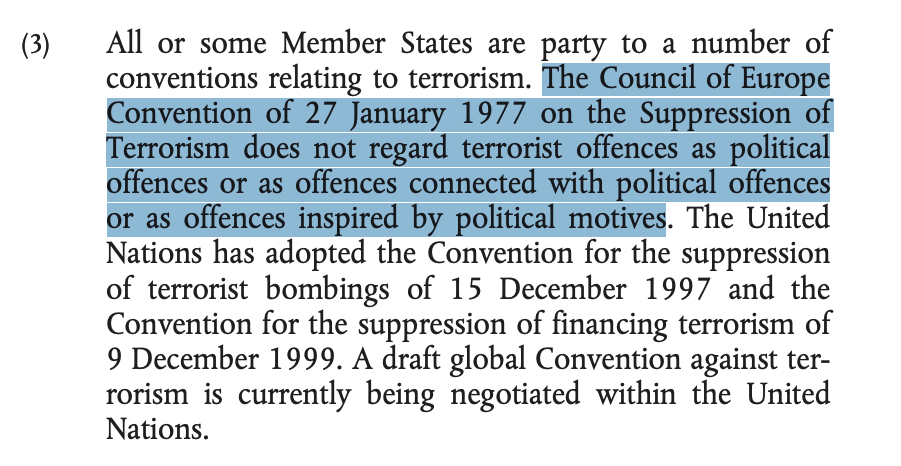
\includegraphics[width = 0.9\textwidth]{../img/eu_law}

Decisión Marco de la UE sobre Terrorismo, 2002

\end{frame}
\note{}
% ----------------------------------------------------

% % ----------------------------------------------------
% \begin{frame}
% \frametitle{Entendiendo el terrorismo}
% \centering

% \begin{itemize}
%   \item[] Esto no vale para entender el fenómeno
%   \begin{itemize}
%     \item<2-> ¿Identificar el terrorismo?
%     \item<3-> ¿Incentivos \red{políticos} para el uso del terrorismo?
%     \item<4-> ¿{\textbf{Quién}} y {\textbf{cuándo}} lo utiliza?
%     \item<5-> ¿Qué significa la \textbf{prevención}? ¿Y cómo la llevamos a cabo?
%   \end{itemize}
% \end{itemize}

% \end{frame}
% \note{}
% % ----------------------------------------------------

% % ----------------------------------------------------
% \imageframe{../img/thiepval_wiki2}
% \note{}
% % ----------------------------------------------------

% ----------------------------------------------------
\begin{frame}
\frametitle{Entendiendo el terrorismo}
\centering

% ----------------------------------------------------
\begin{minipage}{.6\textwidth}\centering
  \begin{itemize}
    \item[] Dos formas de ver esto
    \item<2-> \textbf{Terrorismo} (la acción)
    \visible<3->{\begin{itemize}
      \item ¿Qué es un atentado terrorista?
      \item ¿En qué se diferencia de otras formas de violencia política?
      \item ¿Por qué los actores eligen el terrorismo?
    \end{itemize}}
    \item<2-> \textbf{Terroristas} (el actor)
    \visible<4->{\begin{itemize}
      \item ¿Por qué los actores dependen \textbf{principalmente} del terrorismo?
      \item ¿Cuál es el ``opuesto'' al terrorismo?
    \end{itemize}}
  \end{itemize}
\end{minipage}\hfill
% ----------------------------------------------------
\begin{minipage}{.39\textwidth}\centering
    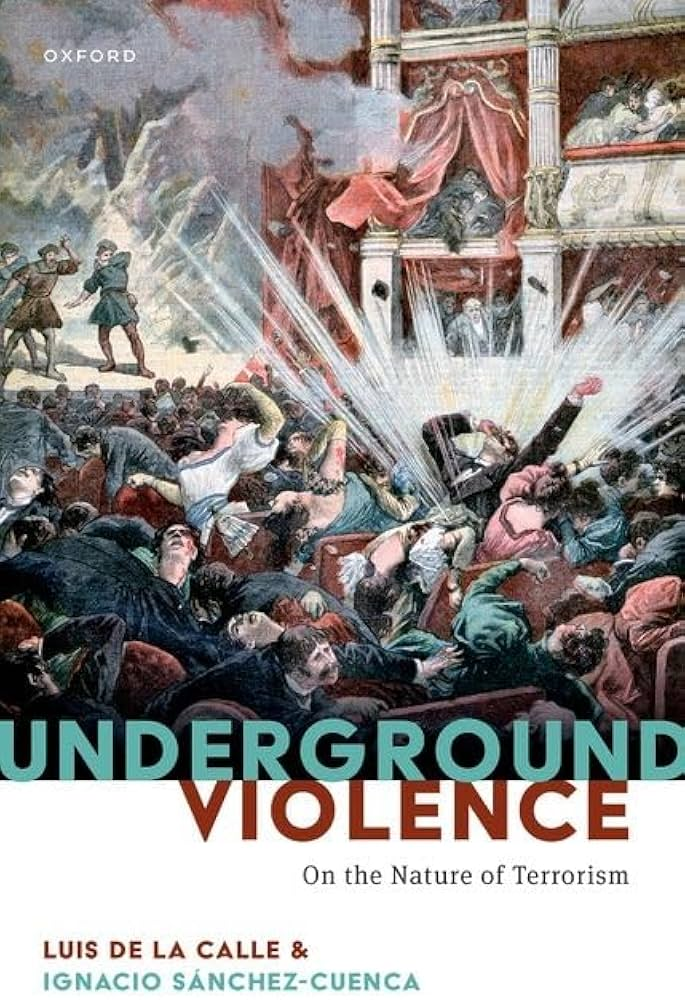
\includegraphics[width = 0.9\textwidth]{../img/underground_violence}\\
    \asher{{\tiny De la Calle \& Sánchez-Cuenca (2024) \textit{Underground Violence: On the Nature of Terrorism.} Oxford U Press.\\}}
\end{minipage}
% ----------------------------------------------------

\end{frame}
\note{}
% ----------------------------------------------------

% ----------------------------------------------------
\begin{frame}[plain]

    \begin{tikzpicture}[remember picture, overlay]
        \node[at = (current page.center), xshift = 0cm, yshift = 1cm] (cover) {%
            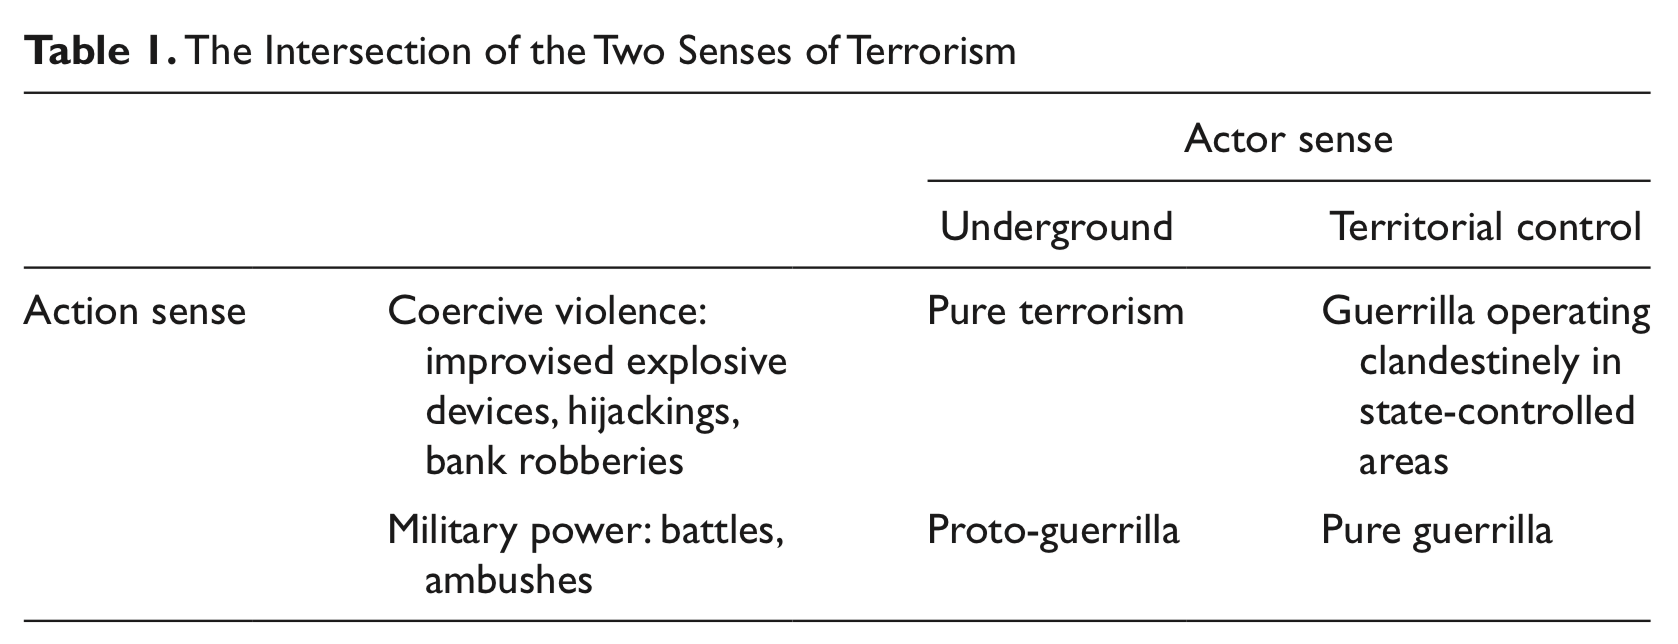
\includegraphics[keepaspectratio, width=\paperwidth, height=\paperheight]{../img/actor-action-sense}
        };
    \end{tikzpicture}

\end{frame}
\note{}
% ----------------------------------------------------

% ----------------------------------------------------
\begin{frame}[plain]

    \begin{tikzpicture}[remember picture, overlay]
        \node[at = (current page.center), xshift = 0cm, yshift = 1cm] (cover) {%
            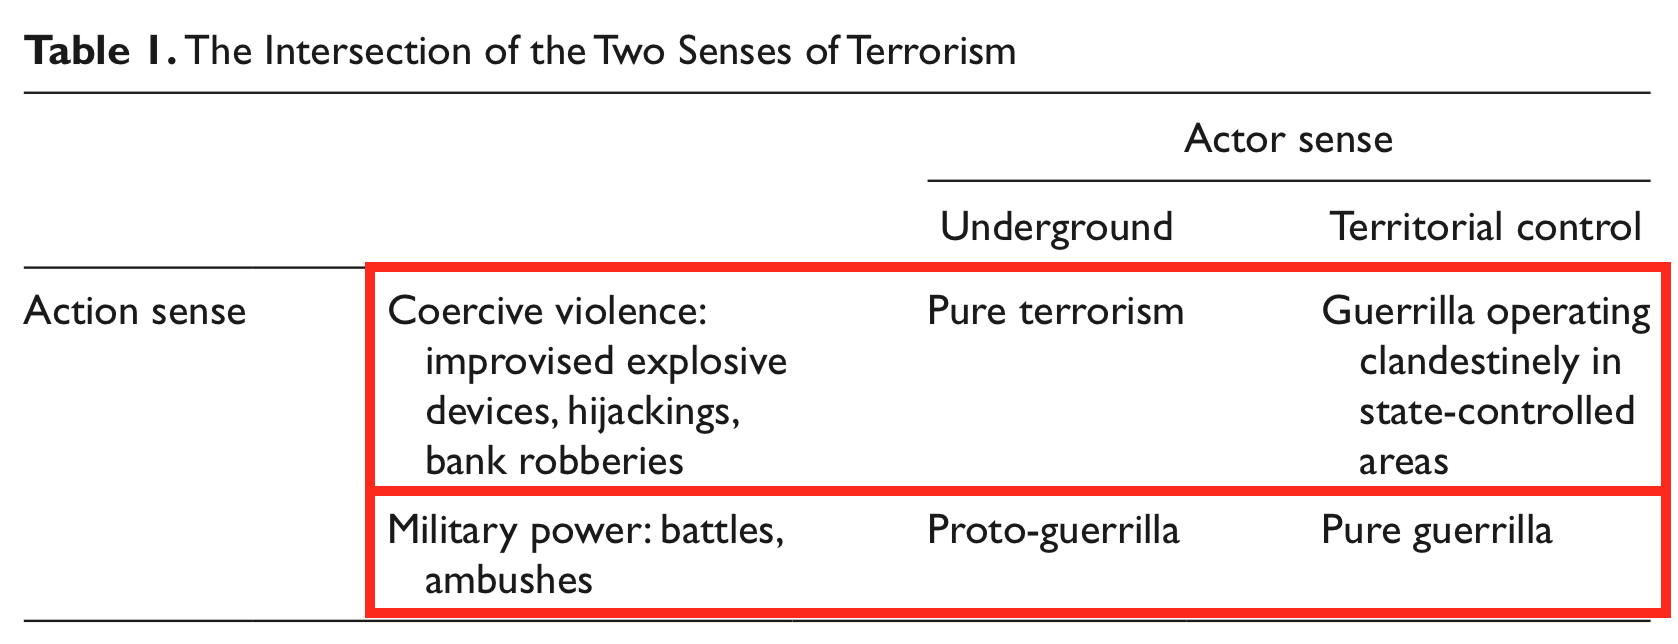
\includegraphics[keepaspectratio, width=\paperwidth, height=\paperheight]{../img/actor-action-sense1}
        };
    \end{tikzpicture}

    \vspace{160pt}

    \begin{itemize}
      \item El terrorismo como una \textbf{acción}:
      \item[] poder militar vs. poder para hacer daño
      \item Naturaleza coercitiva de la violencia terrorista, compatible con tener baja capacidad militar
    \end{itemize}

\end{frame}
\note{}
% ----------------------------------------------------

% ----------------------------------------------------
\begin{frame}[plain]

    \begin{tikzpicture}[remember picture, overlay]
        \node[at = (current page.center), xshift = 0cm, yshift = 1cm] (cover) {%
            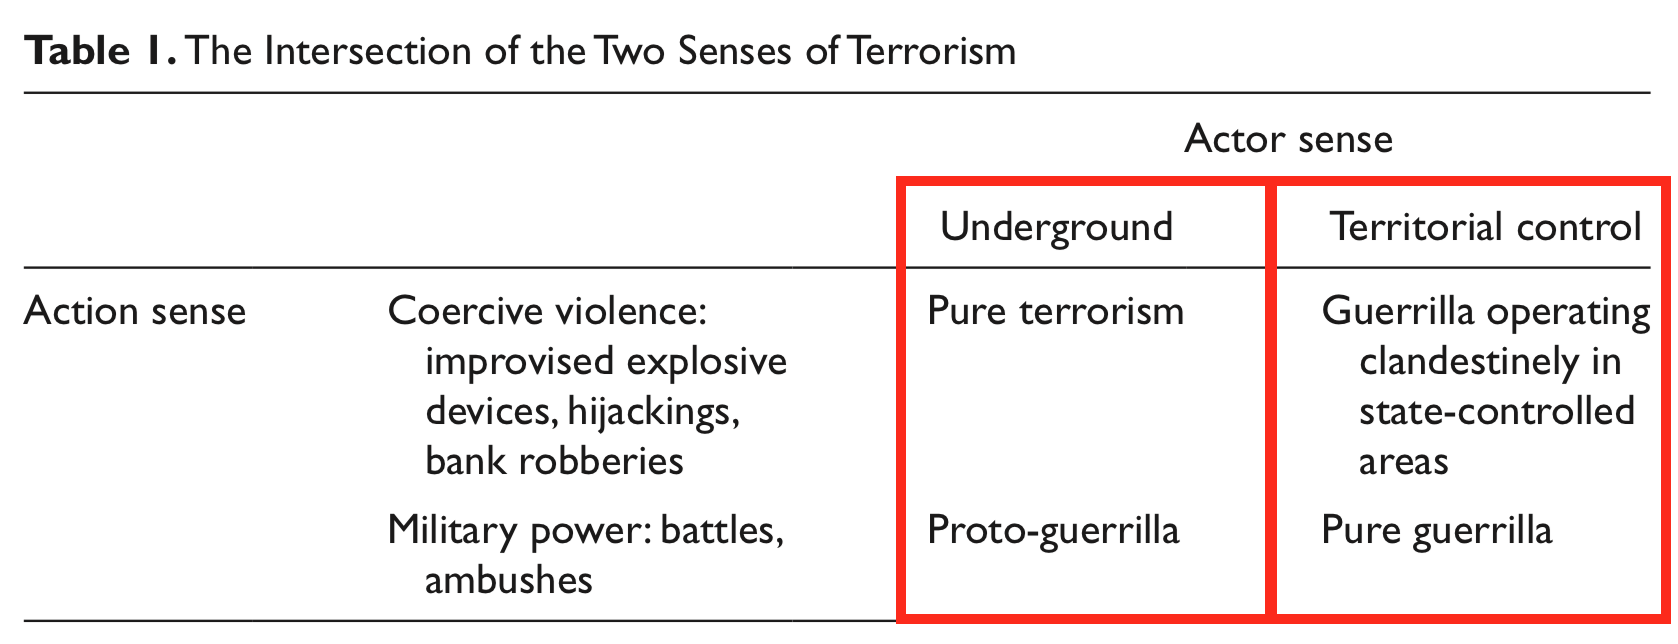
\includegraphics[keepaspectratio, width=\paperwidth, height=\paperheight]{../img/actor-action-sense2}
        };
    \end{tikzpicture}

    \vspace{150pt}

    \begin{itemize}
      \item Los terroristas como \textbf{actores}: grupos clandestinos sin territorio
      \item \textit{Duopolio} de violencia (frente a monopolio fragmentado)
    \end{itemize}

\end{frame}
\note{}
% ----------------------------------------------------

% ----------------------------------------------------
\begin{frame}[plain]

    \begin{tikzpicture}[remember picture, overlay]
        \node[at = (current page.center), xshift = 0cm, yshift = 1cm] (cover) {%
            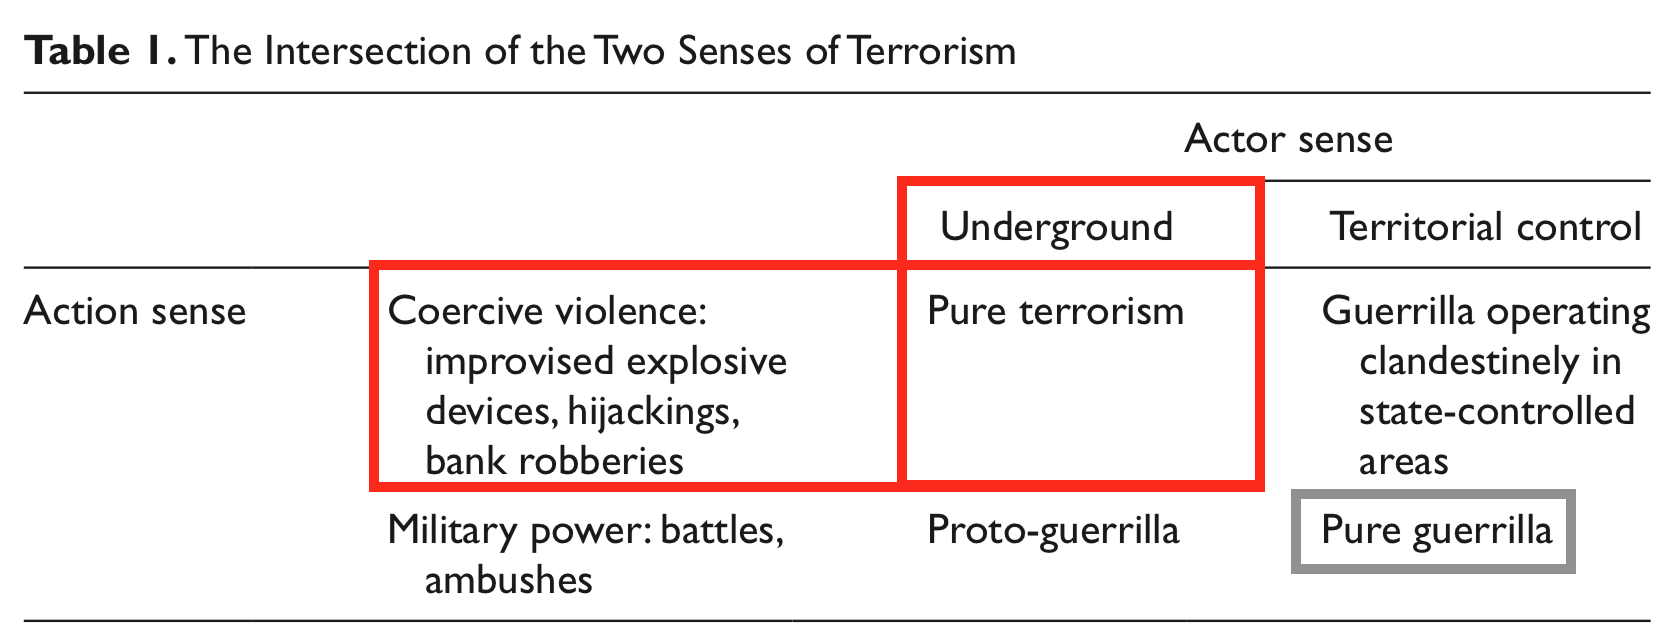
\includegraphics[keepaspectratio, width=\paperwidth, height=\paperheight]{../img/actor-action-sense3}
        };
    \end{tikzpicture}

    \vspace{160pt}

    \begin{itemize}
      \item {\textbf{`Terrorismo puro'}}: grupos clandestinos que usan violencia coercitiva porque no tienen ninguna capacidad militar
      \item<2-> Es fácil distinguir entre tipos ideales (guerrillas y terroristas)
    \end{itemize}

\end{frame}
\note{}
% ----------------------------------------------------

% ----------------------------------------------------
\imageframe{../img/eta-mesa}
\note{}
% ----------------------------------------------------

% ----------------------------------------------------
\imageframe{../img/farc}
\note{}
% ----------------------------------------------------

% ----------------------------------------------------
\begin{frame}[plain]

    \begin{tikzpicture}[remember picture, overlay]
        \node[at = (current page.center), xshift = 0cm, yshift = 1cm] (cover) {%
            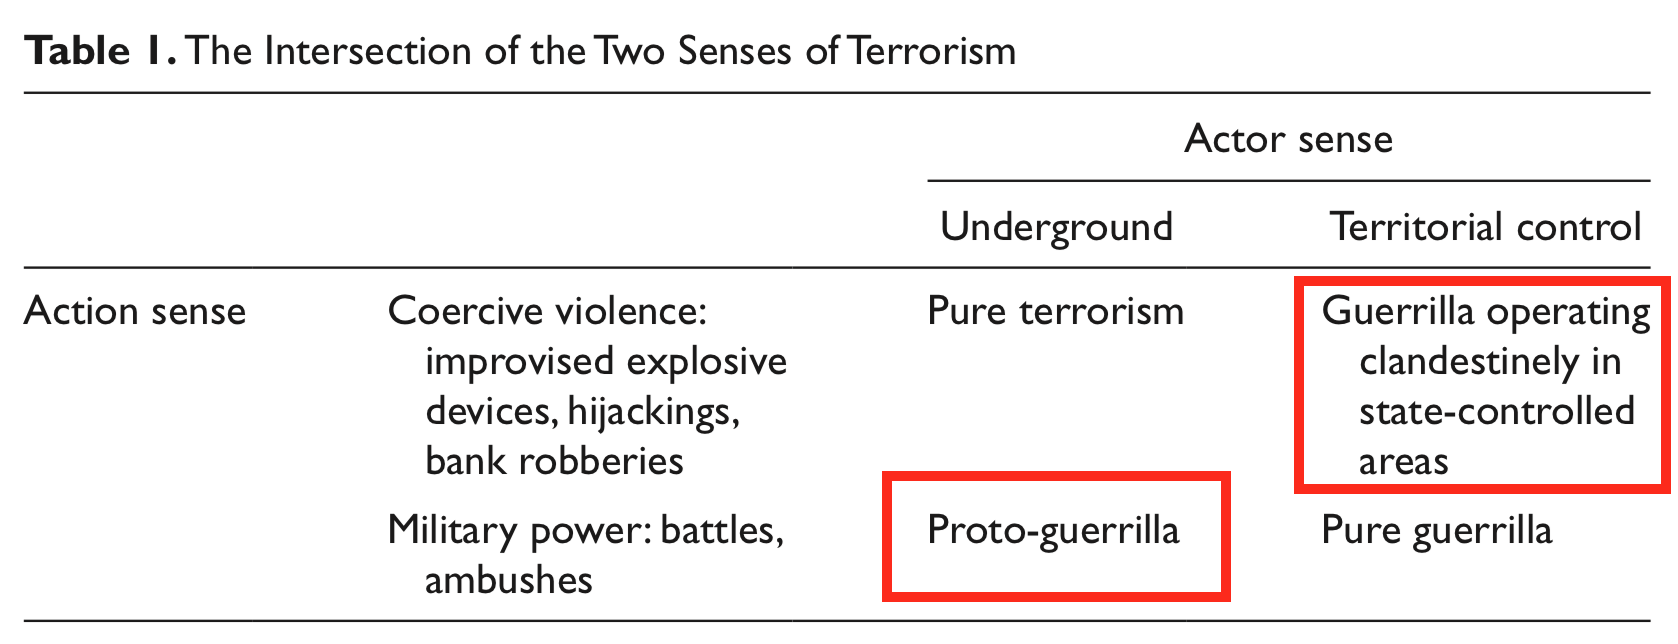
\includegraphics[keepaspectratio, width=\paperwidth, height=\paperheight]{../img/actor-action-sense4}
        };
    \end{tikzpicture}

    \vspace{150pt}

    \begin{itemize}
      \item Pero también existen tipos híbridos, especialmente grupos que controlan territorio \textit{y} emplean violencia terrorista: Sendero Luminoso, PKK, ISIS...
      \item[] (la guerrilla urbana es mucho menos común)
    \end{itemize}

\end{frame}
\note{}
% ----------------------------------------------------

% ----------------------------------------------------
\begin{frame}[plain]

    \begin{tikzpicture}[remember picture, overlay]
        \node[at = (current page.center), xshift = 0cm, yshift = 1cm] (cover) {%
            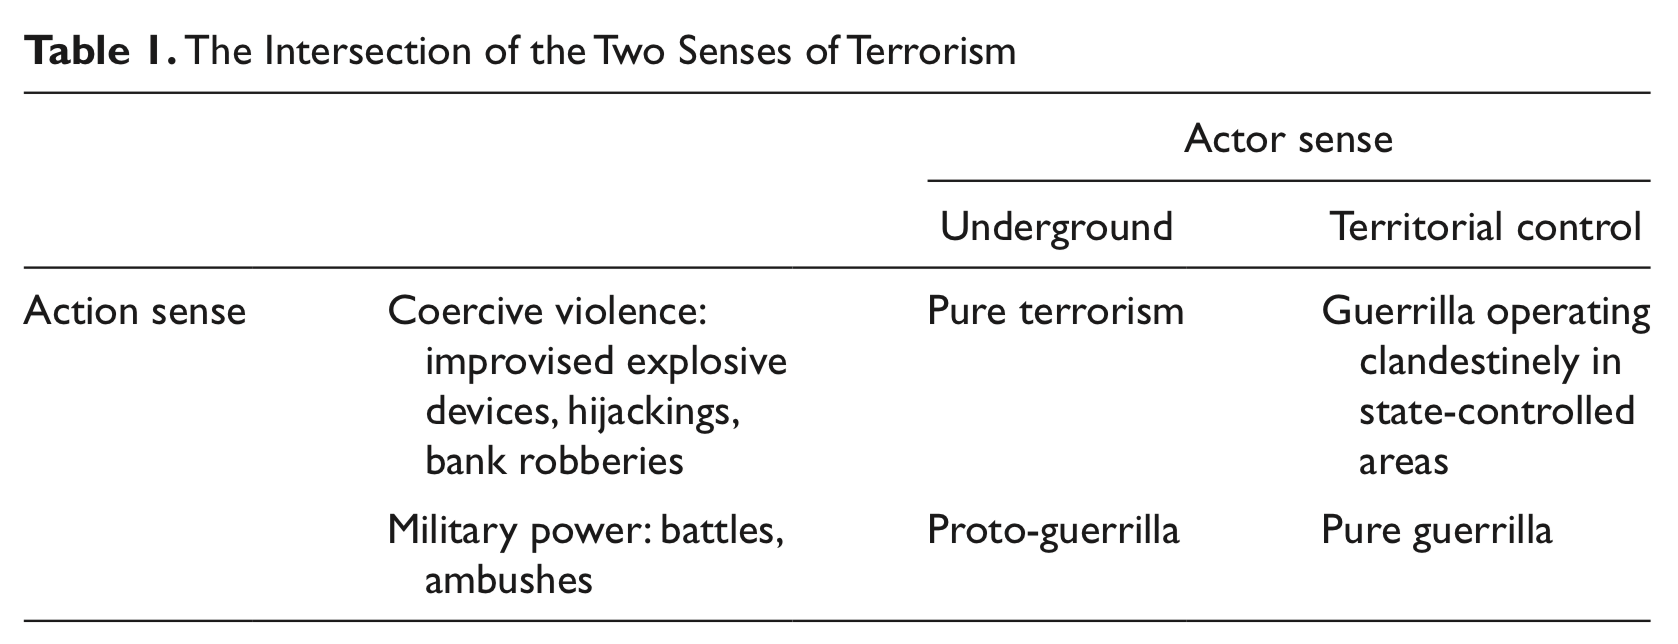
\includegraphics[keepaspectratio, width=\paperwidth, height=\paperheight]{../img/actor-action-sense}
        };
    \end{tikzpicture}

    \vspace{150pt}

    \begin{itemize}
      \item Otras veces cambian de una esquina a otra: Hezbollah (de clandestino a guerrilla), PKK (de guerrilla a clandestino), IRA casi consigue pasar a guerrilla...
    \end{itemize}

\end{frame}
\note{}
% ----------------------------------------------------

% ====================================================
\section{Causas}
% ====================================================

% ----------------------------------------------------
\begin{transitionframe}
Causas
\end{transitionframe}
\note{}
% ----------------------------------------------------

% ----------------------------------------------------
\begin{frame}
\frametitle{¿Por qué estallan las guerras civiles?}
\centering

\begin{minipage}{0.44\textwidth}\centering
  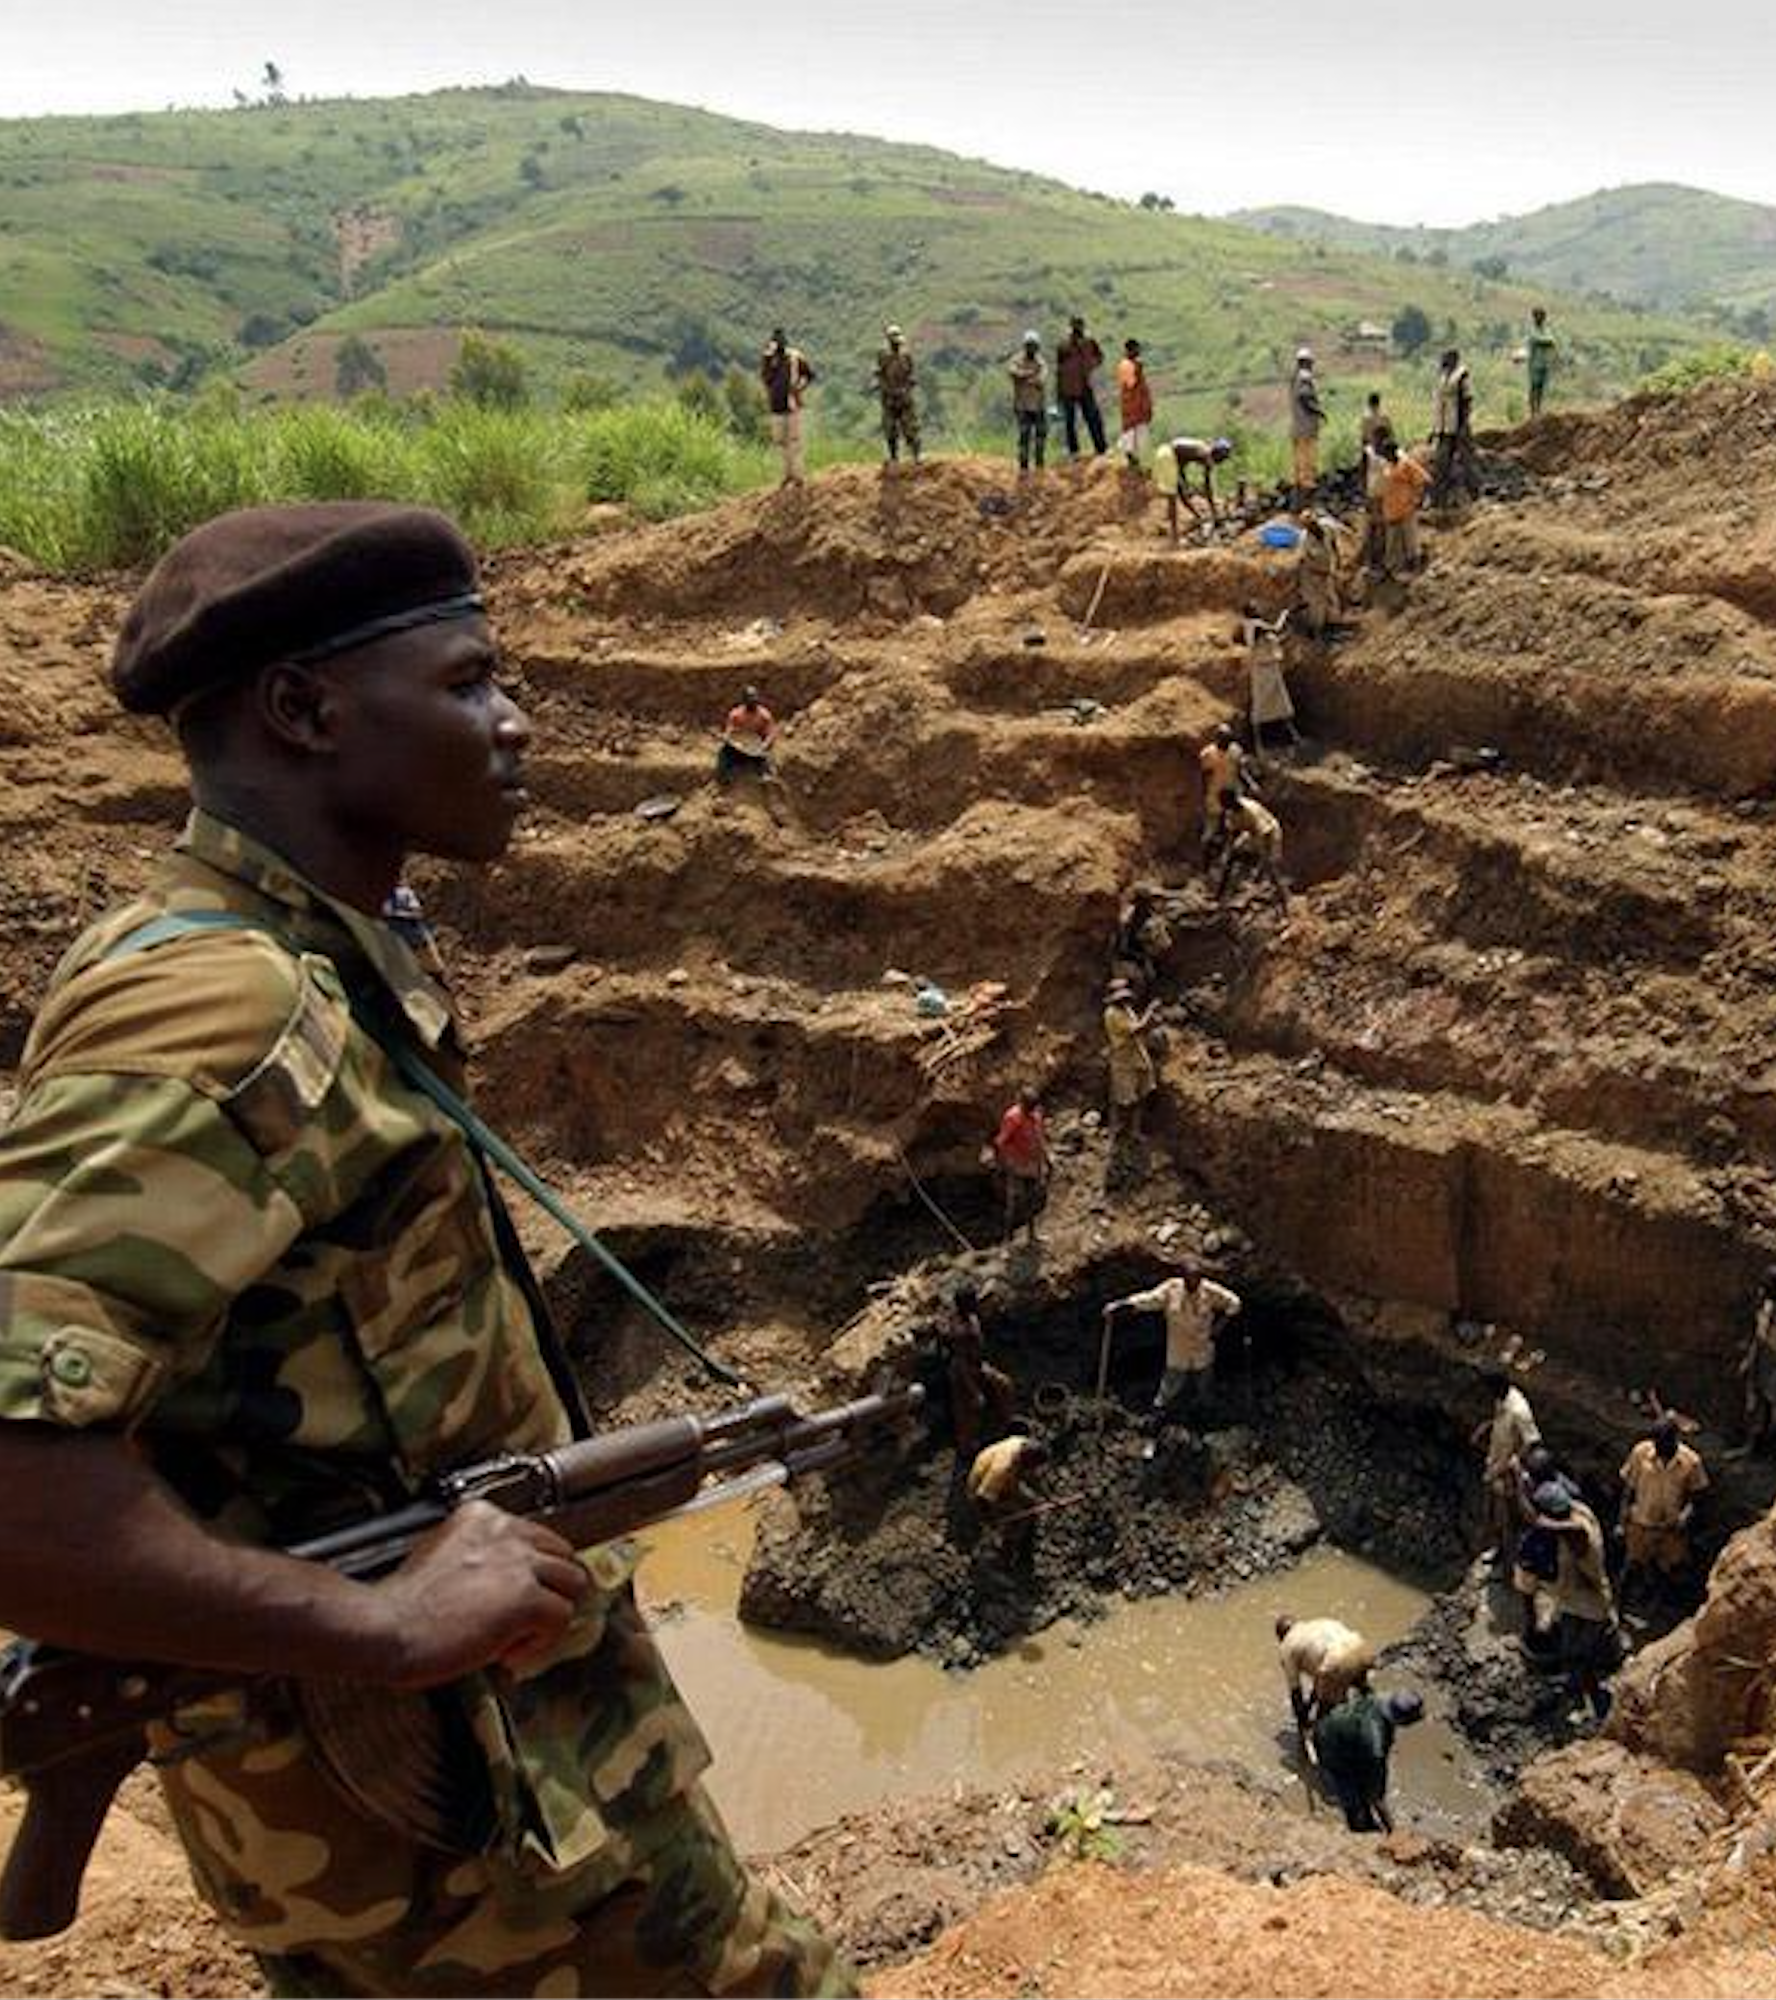
\includegraphics[width = 0.9\textwidth]{../img/conflict_diamonds2}
\end{minipage}
\begin{minipage}{0.44\textwidth}\centering
  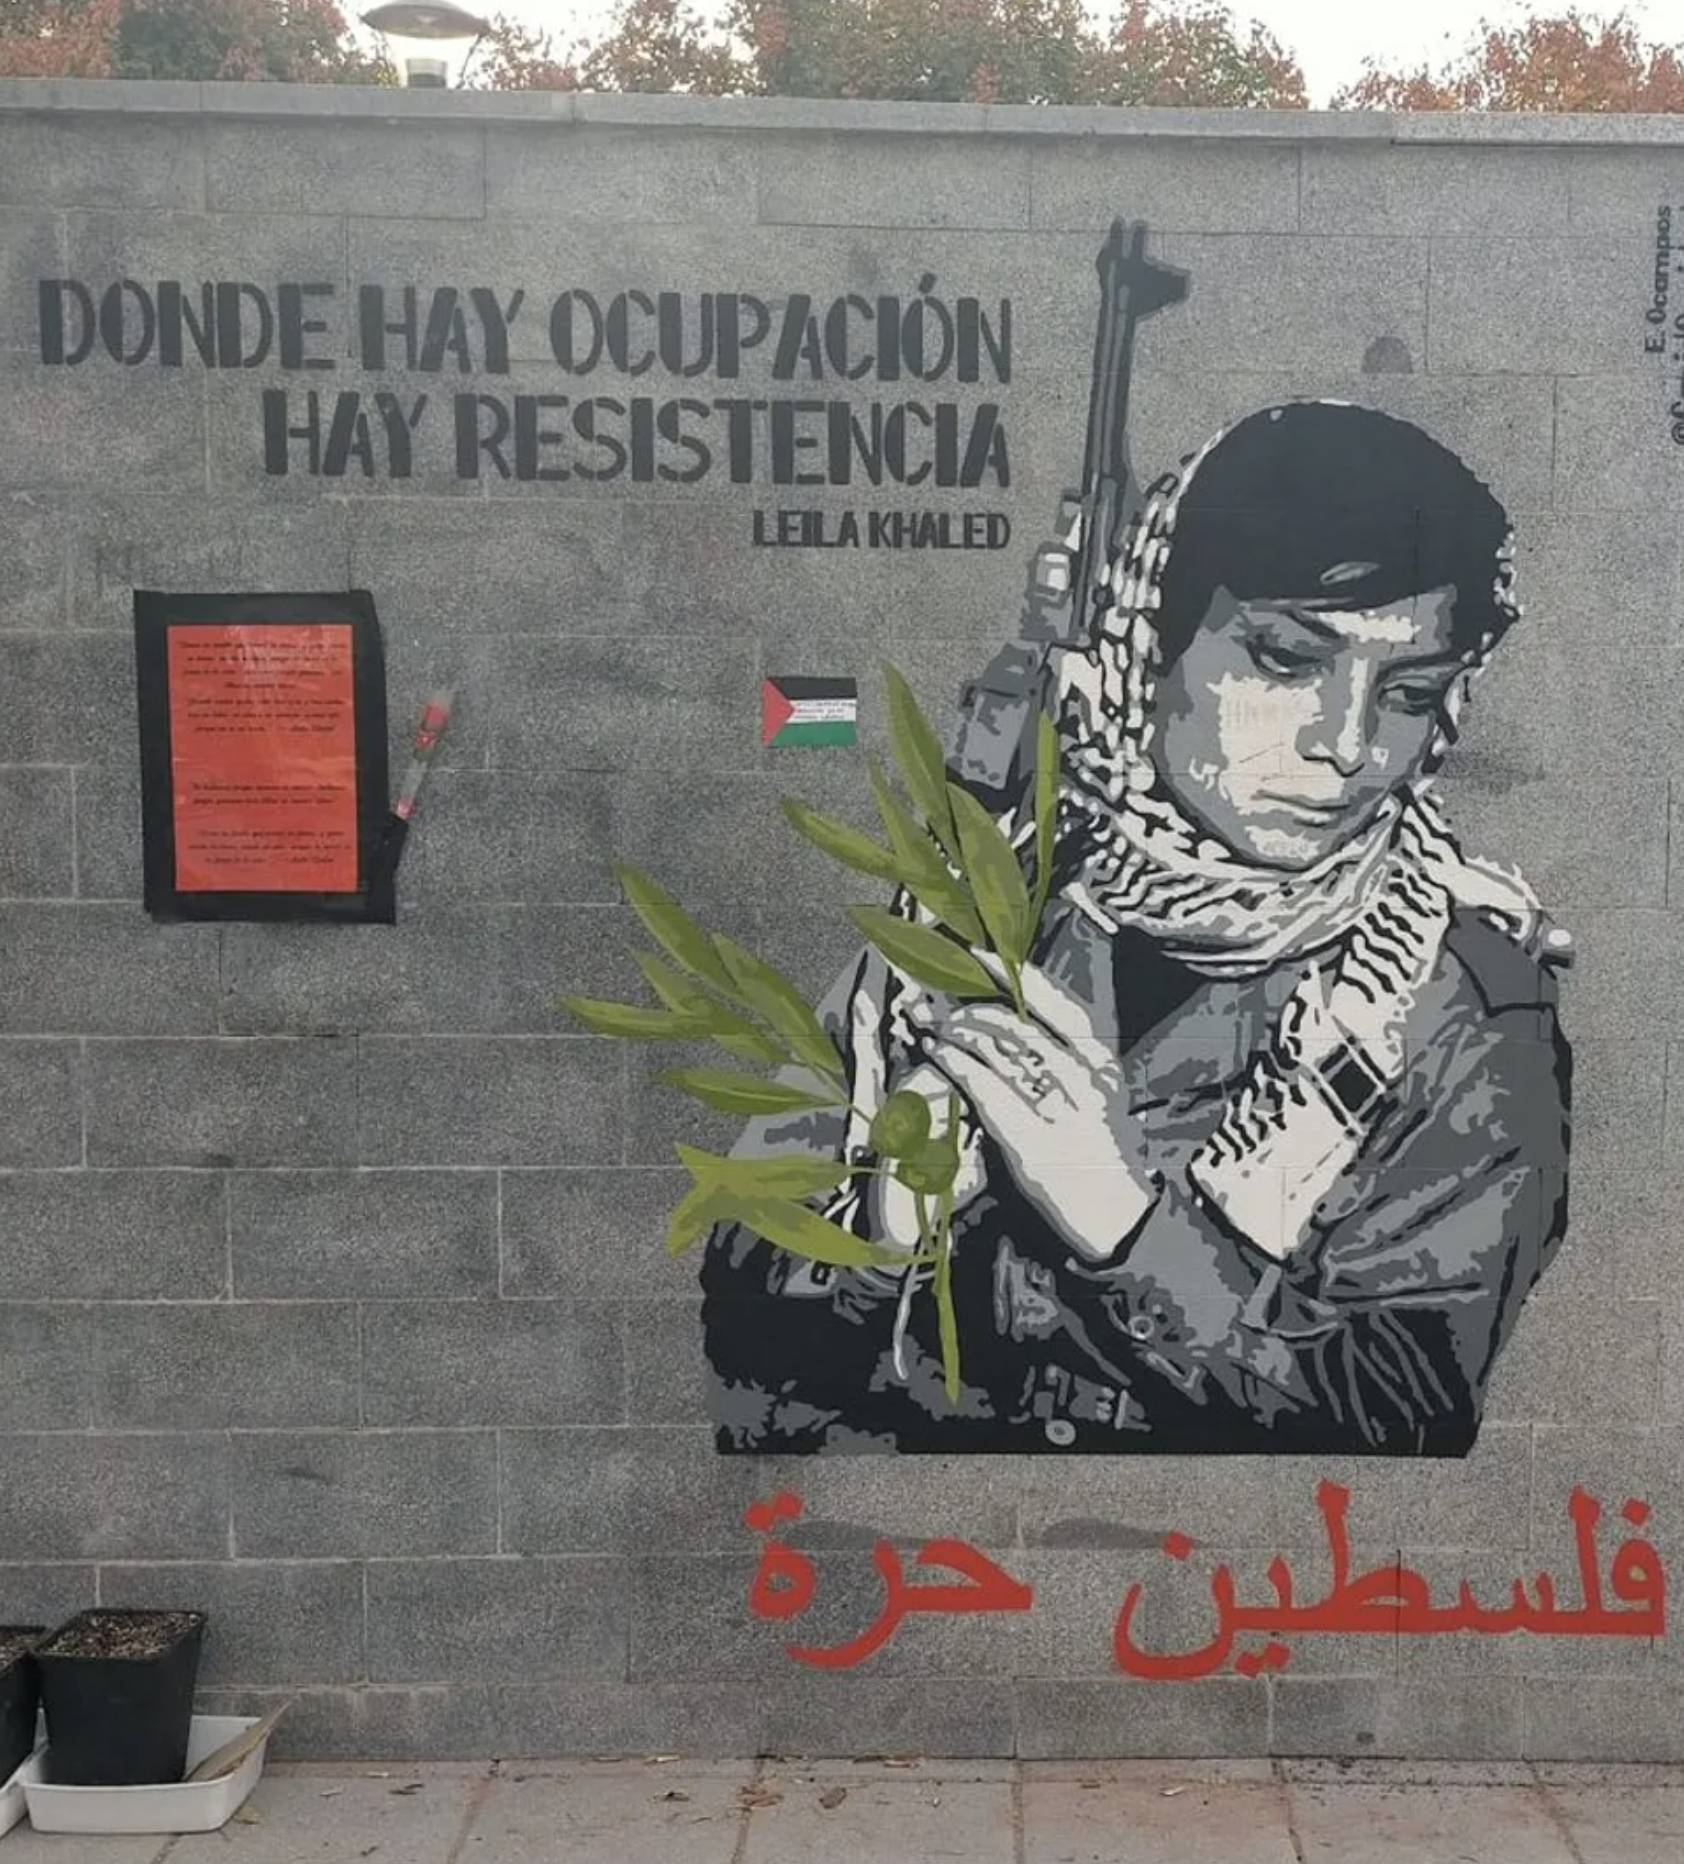
\includegraphics[width = 0.9\textwidth]{../img/mural_palestina}
\end{minipage}

\end{frame}
% ----------------------------------------------------
\note{}

% ----------------------------------------------------
\begin{frame}
\frametitle{Greed vs grievance}
\centering

\begin{columns}[T]
  \begin{column}{0.45\textwidth}
    \centering
    \textbf{\textcolor{accent}{Agravios} (grievances)}
    \begin{itemize}
      \item Exclusión política
      \item Discriminación étnica o religiosa
      \item Represión estatal
      \item {\scriptsize Ej: kurdos en Irak, tutsi en Ruanda}
    \end{itemize}
  \end{column}
  \begin{column}{0.45\textwidth}
    \centering
    \textbf{\textcolor{accent2}{Codicia} (greed)}
    \begin{itemize}
      \item Control de recursos naturales
      \item Diamantes, petróleo, minerales
      \item {\scriptsize Ej: Sierra Leona, Colombia (coca)}
    \end{itemize}
  \end{column}
\end{columns}

\vspace{10pt}
\begin{itemize}
  \item Más correctamente: factores de \textbf{motivación} vs \textbf{oportunidad}
\end{itemize}

\end{frame}
% ----------------------------------------------------
\note{Debate clásico greed vs.~grievance (Collier y Hoeffler vs.~Stewart):
\begin{itemize}
  \item Agravios: discriminación, exclusión del poder político, marginación económica. Ejemplo: los Tutsi en Ruanda, los kurdos en Irak, Turquía y Siria
  \item Codicia: los ``diamantes de sangre'' en Sierra Leona y Liberia, el coltán en Congo, la coca en Colombia. Los recursos naturales pueden financiar la rebelión y crear incentivos económicos para seguir luchando
\end{itemize}
Pero los agravios y la codicia son muy comunes. Lo que falta explicar es por qué en unos casos hay rebelión y en otros no. Para eso necesitamos más factores.}

% ----------------------------------------------------
\begin{frame}
\frametitle{Tres factores que explican la rebelión}
\centering

\begin{itemize}
  \item \textbf{Características del grupo:}
  \begin{itemize}
    \item Lazos étnicos o religiosos fuertes que facilitan la organización
  \end{itemize}
  \item<2-> \textbf{Características del Estado:}
  \begin{itemize}
    \item No democrático, pobre, territorio difícil (montañas, selvas)
    \item Estado débil = más difícil reprimir a los rebeldes
  \end{itemize}
\end{itemize}

\end{frame}
% ----------------------------------------------------
\note{Tres niveles de explicación (análogo a las tres imágenes de Waltz):
\begin{enumerate}
  \item Grupo: las identidades étnicas y religiosas compartidas facilitan superar el problema de acción colectiva. Si el grupo ya tiene redes de confianza, es más fácil reclutar combatientes
  \item Estado: los países pobres y no democráticos son mucho más vulnerables. La pobreza reduce el coste de oportunidad de unirse a la rebelión (pocas alternativas) y debilita la capacidad del Estado para controlar su territorio. Las montañas y las selvas dan refugio a los rebeldes
  \item Internacional: las guerras proxy de la Guerra Fría (Angola, Mozambique, Afganistán, Nicaragua). Hoy: Irán apoya a Hezbolá y a los hutíes; Rusia apoyó a separatistas en Ucrania
\end{enumerate}}

% ----------------------------------------------------
\begin{frame}
\frametitle{Factores internos vs. externos}
\centering

\begin{itemize}
  \item Todas estas explicaciones se centran en factores que varían entre países
  \item Importancia también del sistema internacional
\end{itemize}

\end{frame}
\note{}
% ----------------------------------------------------
  

% ----------------------------------------------------
\begin{frame}
\frametitle{El efecto de la Guerra Fría}
\centering

\begin{itemize}
  % \item ¿Qué hay del efecto del \textit{sistema internacional} en el conflicto interno?
  \item<2-> Cómo los factores globales afectaron a la \textit{tecnología de la rebelión}
  \begin{itemize}
    \item[] {\footnotesize Balcells \& Kalyvas (\textit{APSR}, 2010)}
  \end{itemize}
  \item<3-> Recuerda los tipos:
  \begin{itemize}
    \item Conflictos irregulares (grupos de guerrilla contra ejércitos convencionales)
    \item Guerras civiles convencionales (todos ejércitos convencionales, frentes claros)
    \item No convencionales simétricas
  \end{itemize}
  \item<3-> ¿Afectó el cambio en el sistema internacional (fin de la Guerra Fría) a la forma en que se libran las guerras civiles?
\end{itemize}

\end{frame}
\note{}
% ----------------------------------------------------

% ----------------------------------------------------
\begin{frame}
\frametitle{El efecto de la Guerra Fría (durante y después)}
\centering

\begin{itemize}
  \item Idea principal: el apoyo de las superpotencias en las guerras \textit{proxy} aumentó la capacidad de los insurgentes; por eso vemos tantas guerras irregulares
  \item ¿Cómo? Apoyo material, apoyo ideológico, entrenamiento...
  \item Apoyo a ambos bandos
  \begin{itemize}
    \item P. ej., la URSS apoyó al gobierno de Mozambique y EE. UU. apoyó a RENAMO
  \end{itemize}
  \item<2-> Después de la Guerra Fría, el apoyo de la URSS desaparece y EE. UU. ya no tiene incentivos; los estados previamente existentes colapsan y los ejércitos se fragmentan
  \item<2-> ¿Consecuencia? Aumento de las guerras convencionales y SNC
\end{itemize}

\end{frame}
\note{}
% ----------------------------------------------------


% ----------------------------------------------------
\begin{frame}
\frametitle{El efecto de la Guerra Fría (durante y después)}
\centering

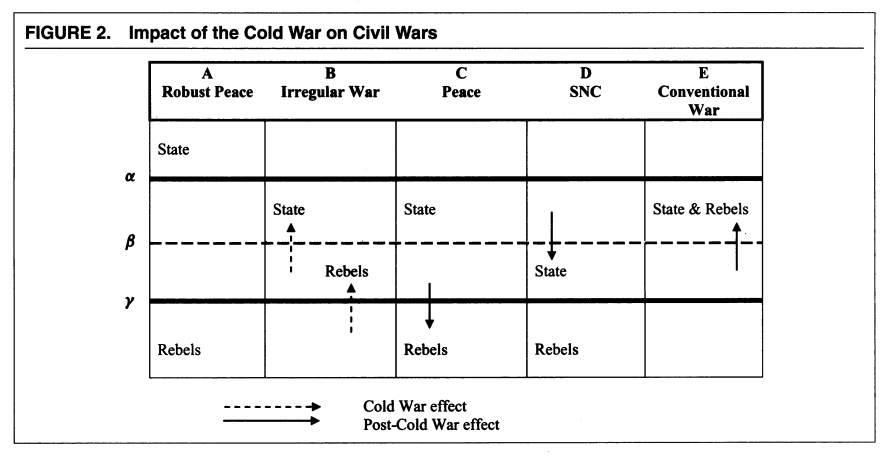
\includegraphics[width = 0.9\textwidth]{../img/kalyvas_balcells_cold_war}

\begin{itemize}
  \item Por encima de $\alpha$: el estado es demasiado fuerte (paz estable)
  \item Por encima de $\beta$: capacidad para usar ejércitos convencionales
  \item Por encima de $\gamma$: capacidad para usar guerra irregular
  \item Por debajo de $\gamma$: capacidad militar insuficiente (bandidos, terroristas, etc.)
\end{itemize}

\end{frame}
\note{}
% ----------------------------------------------------

% ----------------------------------------------------
\begin{frame}
\frametitle{La edad de oro de las \textbf{guerrillas}}
\centering

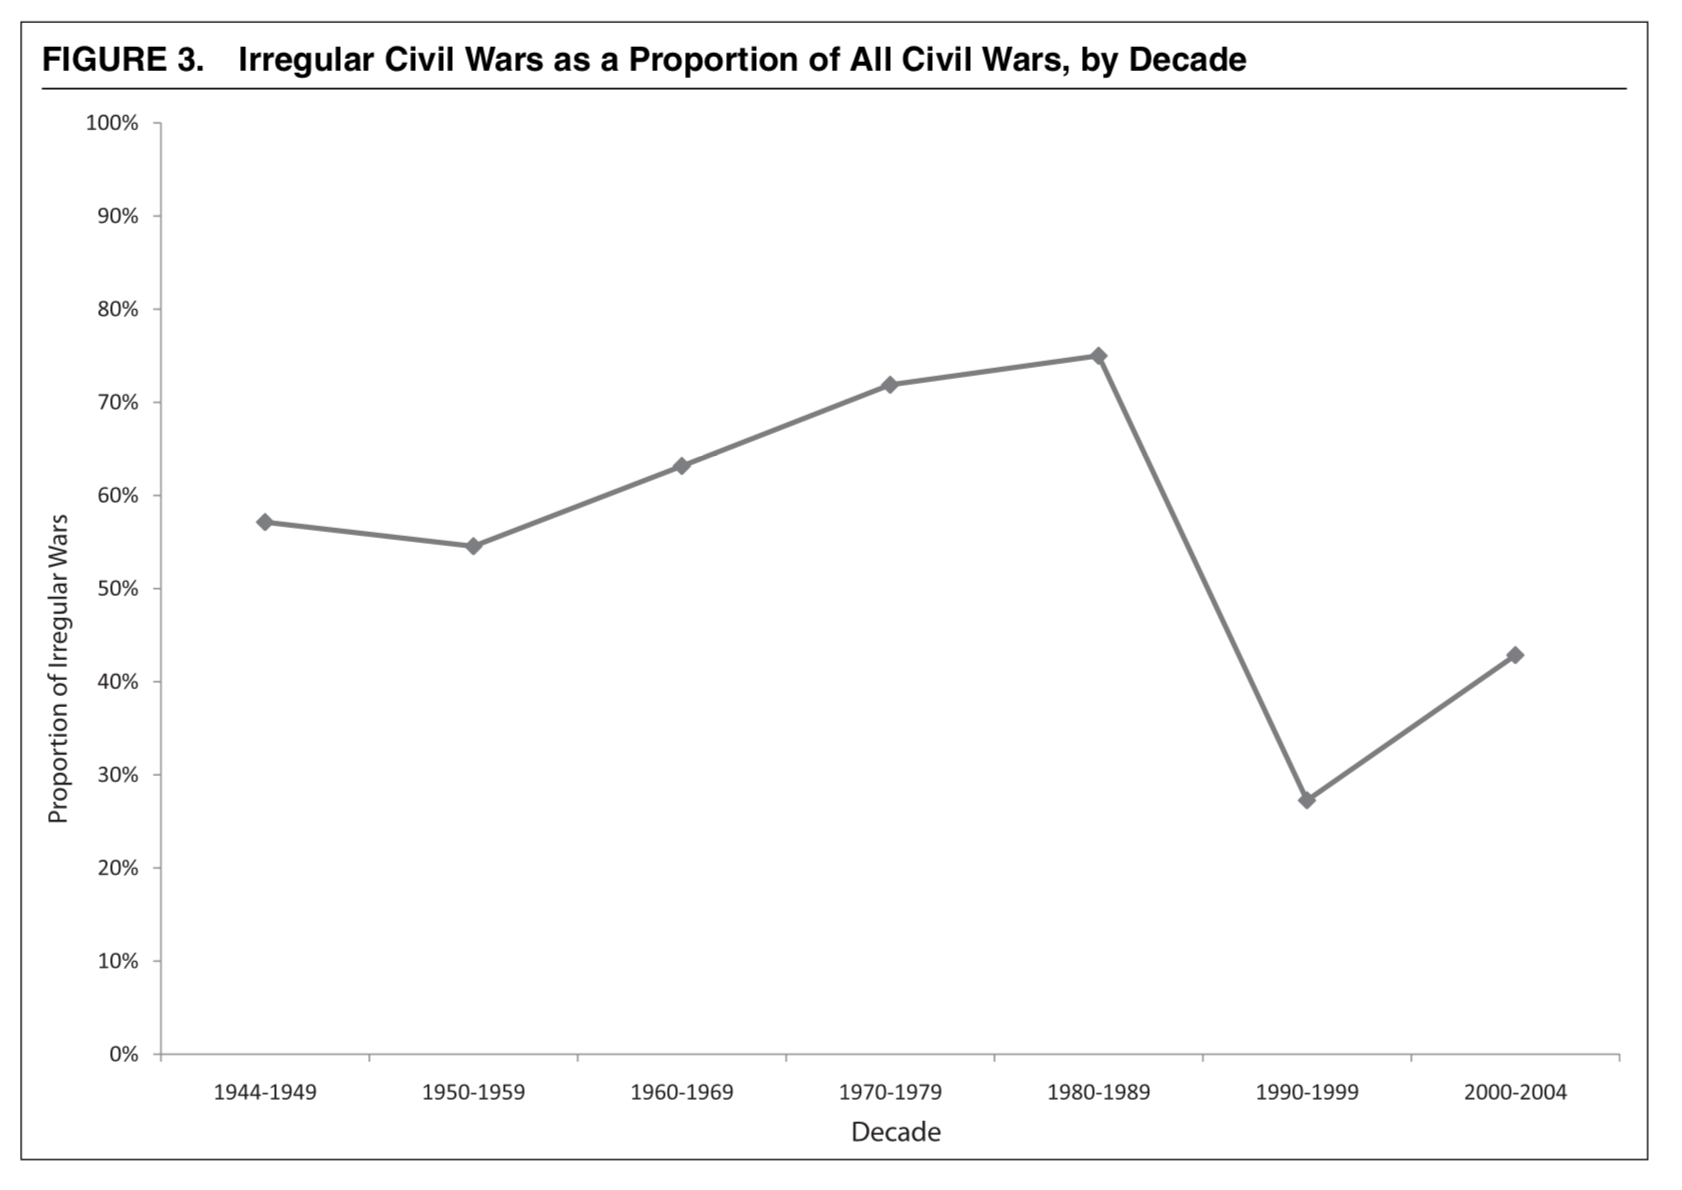
\includegraphics[width = \textwidth]{../img/kalyvas_balcells_irr}

\end{frame}
\note{}
% ----------------------------------------------------

% ====================================================
\section{El desarrollo de las guerras}
% ====================================================

% ----------------------------------------------------
\begin{transitionframe}
Las guerras civiles por dentro
\end{transitionframe}
% ----------------------------------------------------
\note{}

% ----------------------------------------------------
\begin{frame}
\frametitle{Insurgencia y rebeldes}
\centering

\begin{itemize}
  \item Los rebeldes suelen ser más débiles que el Estado
  \item<2-> Recurren a \textbf{guerra asimétrica}:
  \begin{itemize}
    \item Unidades pequeñas, ataques rápidos (\textit{hit-and-run})
    \item Dependen de la población civil
    \item \textbf{Problema de información} en las guerras
  \end{itemize}
  \item<3-> Dos objetivos/consecuencias al mezclarse con civiles:
  \begin{itemize}
    \item Evitar ser detectados
    \item Provocar que el gobierno ataque a civiles $\rightarrow$ ganan apoyo
  \end{itemize}
\end{itemize}

\end{frame}
% ----------------------------------------------------
\note{La insurgencia es la forma de guerra más común en el mundo. Los rebeldes no tienen los recursos para enfrentarse al ejército del Estado en batalla abierta, así que usan tácticas de guerrilla:
\begin{itemize}
  \item Emboscadas, sabotaje, ataques a instalaciones
  \item Se esconden entre los civiles: un insurgente puede ser un granjero por el día y un combatiente por la noche
  \item Si el gobierno responde con violencia indiscriminada contra civiles, la población se aliena del gobierno y apoya a los rebeldes. Esto es una estrategia deliberada de los insurgentes
\end{itemize}
Mao Zedong: ``El guerrillero se mueve entre la gente como un pez en el agua.'' Vietnam, Afganistán, Irak -- todos ejemplos de cómo los insurgentes explotan la ventaja del terreno y la población.}

% ----------------------------------------------------
\begin{frame}
\frametitle{Contrainsurgencia (COIN)}
\centering

\begin{itemize}
  \item \textbf{COIN:} conjunto de estrategias para combatir la insurgencia
  \item<2-> No basta con superioridad militar:
  \begin{itemize}
    \item Hay que ``ganar los corazones y las mentes''
    \item Proporcionar seguridad y servicios a la población civil
    \item Separar a los insurgentes de su base social
  \end{itemize}
  \item<3-> Difícil, y conlleva muchas vidas humanas
\end{itemize}

\end{frame}
% ----------------------------------------------------
\note{La contrainsurgencia (COIN) es la respuesta del Estado a la insurgencia. La doctrina moderna (Petraeus en Irak, McChrystal en Afganistán) enfatiza:
\begin{itemize}
  \item Proteger a la población civil, no solo perseguir a los insurgentes
  \item Proporcionar servicios básicos (seguridad, justicia, economía)
  \item Construir la legitimidad del Estado local
\end{itemize}
Pero es extremadamente difícil, especialmente para un ejército extranjero:
\begin{itemize}
  \item EE.UU. en Vietnam (1955-75): 20 años, 58.000 muertos americanos, derrota
  \item EE.UU. en Afganistán (2001-21): 20 años, billones de dólares, colapso del gobierno afgano al retirarse
  \item Irak: la ``surge'' de 2007 tuvo éxito temporal, pero la inestabilidad continuó
\end{itemize}}

% ----------------------------------------------------
\begin{frame}
\frametitle{Civiles: violencia colateral?}
\centering

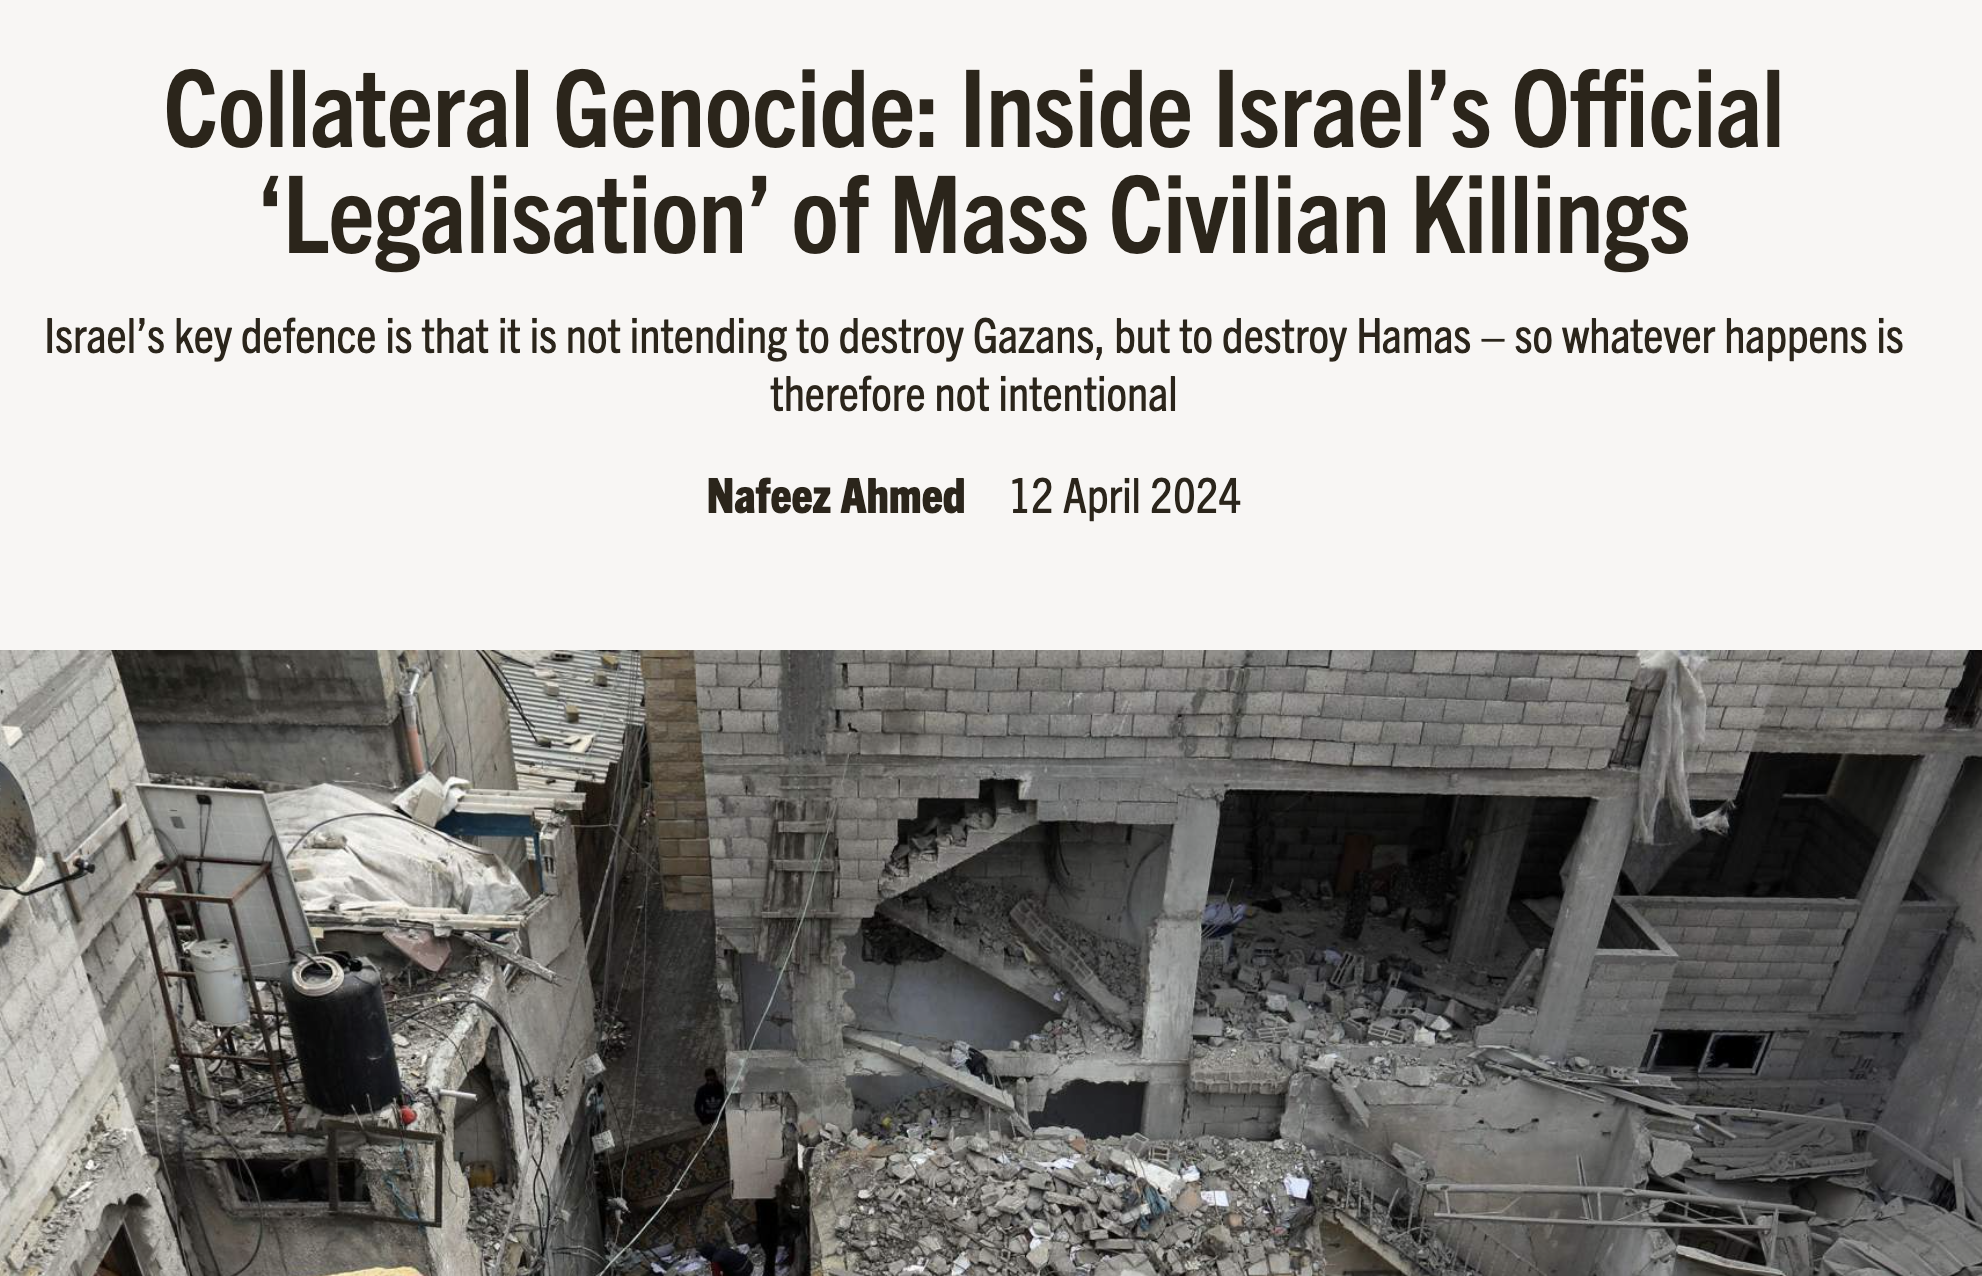
\includegraphics[width = \textwidth]{../img/gaza}
  
\end{frame}
\note{}
% ----------------------------------------------------

% ----------------------------------------------------
\begin{frame}
\frametitle{Violencia contra civiles}
\centering

\begin{itemize}
    \item Lógica estratégica, que tiene mucho que ver con la \textbf{lógica de la insurgencia}
    \begin{itemize}
        \item Poca distinción civiles/militares, apoyo de la población etc
        \item Guerras irregulares vs convencionales
    \end{itemize}
    \item<2-> Violencia como coacción vs violencia para castigar al enemigo
    \item<3-> Factores de \textit{constraint} a nivel de grupo
    \item<4-> Dinámicas locales: control territorial, ideología
    \item<5-> Guerras étnicas vs no-étnicas (ideológicas)
\end{itemize}

\end{frame}
\note{}
% ----------------------------------------------------
  


% ----------------------------------------------------
\begin{frame}
\frametitle{¿Por qué duran tanto las guerras civiles?}
\centering

\begin{itemize}
  \item Las guerras civiles duran, de media, \textbf{mucho más} que las interestatales
  \item<2-> ¿Por qué?
  \item<2-> Los mismos problemas de negociación, pero \textbf{agravados}
  \begin{itemize}
    \item Información incompleta
    \item Problemas de compromiso (especialmente graves)
    \item Bienes indivisibles
  \end{itemize}
\end{itemize}

\end{frame}
% ----------------------------------------------------
\note{Las guerras civiles duran una media de 7-10 años, frente a unos pocos meses o años de las interestatales. ¿Por qué?

Aplicamos el modelo de negociación:
\begin{itemize}
  \item Información incompleta: los rebeldes operan en la clandestinidad. Es muy difícil conocer su fuerza real, su organización, su cohesión
  \item Problemas de compromiso: este es el factor clave. Si los rebeldes se desarman como parte de un acuerdo de paz, ¿qué les garantiza que el gobierno cumplirá? Un ejército desarmado es un ejército indefenso
  \item Indivisibilidad: cuando un gobierno enfrenta a múltiples grupos separatistas, ceder ante uno puede animar a otros. Esto hace que cada concesión sea más costosa
\end{itemize}
Resultado: las guerras civiles rara vez terminan con acuerdos negociados. Lo más común es la victoria militar de un bando.}

% ----------------------------------------------------
\begin{frame}
\frametitle{El problema de compromiso en guerras civiles}
\centering

\begin{itemize}
  \item Si los rebeldes se desarman:
  \begin{itemize}
    \item ¿Quién les protege si el gobierno no cumple?
  \end{itemize}
  \item<2-> Si el gobierno hace concesiones:
  \begin{itemize}
    \item ¿Puede garantizar que \textit{todos} los rebeldes dejarán las armas?
  \end{itemize}
  \item<3-> Solución: involucrar a \textbf{terceros} (peacekeepers)
  \begin{itemize}
    \item Monitorear y hacer cumplir los acuerdos
  \end{itemize}
\end{itemize}

\end{frame}
% ----------------------------------------------------
\note{El problema de compromiso es especialmente grave en guerras civiles porque no hay separación geográfica como entre Estados:
\begin{itemize}
  \item Los rebeldes no pueden retirarse ``a su territorio'' -- viven dentro del Estado
  \item Si se desarman, quedan a merced del gobierno. El gobierno tiene incentivos para renegar una vez los rebeldes estén desarmados
  \item Por el lado del gobierno: los movimientos rebeldes suelen tener facciones. Incluso si el líder firma un acuerdo, facciones disidentes pueden seguir luchando
\end{itemize}
Por esto los peacekeepers de la ONU son tan importantes: actúan como garantes neutrales del acuerdo. La evidencia muestra que los acuerdos de paz con peacekeepers tienen más probabilidad de durar.}


% ----------------------------------------------------
\begin{frame}
\frametitle{Dos casos de problema de compromiso}
\centering

\begin{itemize}
    \item[1.] Conflictos `sons-of-the-soil'
    \begin{itemize}
        \item `Indígenas' vs migrantes de otras partes del país
        \item Problema de cambios demográficos, credibilidad del estado central
        \item NE India (Assam), Chittagong Hills en Bangladesh, Tamiles en Sri Lanka, Uighurs en China, Cisjordania...
    \end{itemize}
    \item<2->[2.] Guerras civiles donde se financian con contrabando
    \begin{itemize}
        \item Si negocian la paz, pierden fuente de recursos
        \item Drogas, piedras preciosas, etc
        \item FARC y la cocaína, Talibanes y opio, DRC y minerales...
    \end{itemize}
\end{itemize}

\end{frame}
\note{}
% ----------------------------------------------------

% ----------------------------------------------------
\begin{transitionframe}
Entendiendo el terrorismo
\end{transitionframe}
% ----------------------------------------------------
\note{}

% ----------------------------------------------------
\begin{frame}
\frametitle{¿Por qué el terrorismo?}
\centering

\begin{itemize}
  \item Los grupos terroristas son mucho más \textbf{débiles} que los Estados
  \item Sus objetivos son \textbf{desproporcionados} respecto a sus capacidades
  \begin{itemize}
    \item Por eso son débiles: suelen estar lejos del status quo
  \end{itemize}
  \item<2-> El terrorismo es una estrategia del \textbf{débil contra el fuerte}
  \begin{itemize}
    \item Imponer costes para forzar concesiones
    \item Compensar la desventaja militar convencional
    \item Movilizar apoyo de la población
  \end{itemize}
\end{itemize}

\end{frame}
% ----------------------------------------------------
\note{El terrorismo se entiende como resultado de una asimetría de poder extrema. Si los grupos tuvieran capacidad militar convencional, lucharían una guerra convencional. Como no la tienen, recurren a tácticas que:
\begin{itemize}
  \item Maximizan el impacto psicológico y mediático con recursos mínimos
  \item Explotan la vulnerabilidad inherente de las sociedades abiertas
  \item Imponen costes desproporcionados al Estado (la ``guerra contra el terror'' ha costado billones de dólares a EE.UU.)
\end{itemize}
Los 19 secuestradores del 11-S usaron cortaplumas para causar casi 3.000 muertos y provocar una respuesta que ha costado más de 8 billones de dólares.}

% ----------------------------------------------------
\begin{frame}
\frametitle{Cuatro estrategias terroristas}
\centering

\footnotesize
\begin{tabular}{>{\bfseries}l p{6.0cm}}
Coerción & Imponer costes al enemigo para forzar concesiones \\[4pt]
\onslide<2->{Provocación & Provocar una respuesta desproporcionada del Estado que aliene a la población} \\[4pt]
\onslide<3->{Spoiling & Sabotear un proceso de paz que perjudica al grupo} \\[4pt]
\onslide<4->{Outbidding & Competir con otros grupos por el apoyo de la misma base social} \\
\end{tabular}

\end{frame}
% ----------------------------------------------------
\note{Cuatro estrategias (Kydd y Walter, 2006):
\begin{enumerate}
  \item Coerción: la más directa. Atacar para que el enemigo prefiera ceder a seguir sufriendo. Hezbolá atacó barracones de Marines en Beirut (1983): EE.UU. se retiró de Líbano
  \item Provocación: atacar para que el Estado responda con violencia indiscriminada, lo que radicaliza a la población y genera nuevos reclutas para los terroristas. Bin Laden buscaba provocar una invasión de tierras musulmanas para movilizar a la \textit{umma}. El 11-S provocó exactamente eso
  \item Spoiling: cuando moderados de ambos bandos están cerca de un acuerdo, los extremistas atacan para descarrilarlo. Hamas y los ataques suicidas durante los procesos de paz israelí-palestinos. Hamas el 7 de octubre de 2023, saboteando la normalización con Arabia Saudí
  \item Outbidding: cuando varios grupos compiten por representar la misma causa, atacar demuestra quién es más ``comprometido''. Varias facciones palestinas compitiendo entre sí
\end{enumerate}}

% ----------------------------------------------------
\begin{frame}
\frametitle{Ejemplo: el 11-S y las cuatro estrategias}
\centering

\footnotesize
\begin{itemize}
  \item \textbf{Coerción:} forzar la retirada de EE.UU. de Oriente Medio
  \item<2-> \textbf{Provocación:} provocar una invasión de tierras musulmanas que radicalice a millones
  \item<3-> \textbf{Spoiling:} impedir cualquier normalización entre EE.UU. y regímenes árabes moderados
  \item<4-> \textbf{Outbidding:} demostrar que Al Qaeda era el grupo más ``comprometido'' del yihadismo global
\end{itemize}

\vspace{8pt}
\onslide<5->{\footnotesize ¿Cuál fue la estrategia principal de Bin Laden? ¿Funcionó?}

\end{frame}
% ----------------------------------------------------
\note{Ejemplo concreto que aplica las cuatro estrategias a un caso real. Según la mayoría de los analistas, la estrategia principal de Bin Laden era la \textbf{provocación}: quería que EE.UU. invadiera países musulmanes, lo que radicalizaría a la población y generaría una ola de reclutamiento. En cierto sentido funcionó: las guerras de Irak y Afganistán generaron un enorme antiamericanismo y facilitaron el surgimiento del Estado Islámico. Pero Al Qaeda como organización fue gravemente debilitada. La coerción fracasó: EE.UU. no se retiró, sino que aumentó su presencia. El outbidding funcionó parcialmente: Al Qaeda se posicionó como líder del yihadismo global, pero luego fue superada por el ISIS.}

% % ----------------------------------------------------
% \begin{frame}
% \frametitle{¿Por qué falla la negociación con terroristas?}
% \centering

% \begin{itemize}
%   \item \textbf{Información incompleta:}
%   \begin{itemize}
%     \item Los grupos son clandestinos; incentivos para exagerar su fuerza
%   \end{itemize}
%   \item<2-> \textbf{Problemas de compromiso:}
%   \begin{itemize}
%     \item Si se desarman, quedan expuestos
%     \item El gobierno no puede confiar en que \textit{todos} los miembros respetarán el acuerdo
%   \end{itemize}
%   \item<3-> \textbf{Bienes indivisibles:}
%   \begin{itemize}
%     \item Los objetivos suelen ser extremos (califato, destrucción de un Estado)
%   \end{itemize}
% \end{itemize}

% \end{frame}
% % ----------------------------------------------------
% \note{Las mismas tres causas del fracaso en la negociación, pero con características especiales:
% \begin{enumerate}
%   \item Información: los grupos terroristas operan en la clandestinidad. Es extremadamente difícil conocer su tamaño, capacidad y cohesión interna. Los terroristas tienen incentivos para parecer más fuertes de lo que son (para que el gobierno haga más concesiones)
%   \item Compromiso: si un grupo terrorista se desarma y entra en la política, queda vulnerable a la represión. El gobierno puede renegar. Por otro lado, los líderes terroristas a menudo no controlan a todas las facciones de su grupo
%   \item Indivisibilidad: los objetivos de muchos grupos terroristas involucran valores que no se pueden negociar fácilmente: un califato islámico, la destrucción de Israel, etc. Aunque estos objetivos extremos también pueden ser posiciones negociadoras exageradas
% \end{enumerate}}

% ----------------------------------------------------
\begin{frame}
\frametitle{Entendiendo el \textit{surgimiento} del terrorismo}
\centering

\begin{itemize}
  \item[1.] \textbf{Capacidad del estado}
  \begin{itemize}
    \item Recuerda el inicio de las guerras civiles y la capacidad estatal
    \item Los terroristas son las guerrillas de los países más ricos
  \end{itemize}
  \item<2->[2.] \textbf{Tipo de régimen}
  \begin{itemize}
    \item Relación en forma de «U» entre los regímenes represivos/democráticos y el inicio del terrorismo
  \end{itemize}
  \item<3->[3.] \textbf{Trayectoria histórica}
  \begin{itemize}
    \item La Europa de entreguerras y el terrorismo después de los años 60/70
    \item[] {\scriptsize (En países con una trayectoria no liberal, la izquierda estaba más radicalizada; sin embargo, en los países liberales, el apoyo social [de izquierdas] a la violencia era mucho menor $\rightarrow$ moderación de los grupos armados)}
  \end{itemize}
\end{itemize}

\end{frame}
\note{}
% ----------------------------------------------------

% % ====================================================
% \section{Respuestas al terrorismo}
% % ====================================================

% % ----------------------------------------------------
% \begin{transitionframe}
% ¿Qué pueden hacer los Estados ante el terrorismo?
% \end{transitionframe}
% % ----------------------------------------------------
% \note{}

% ----------------------------------------------------
\begin{frame}
\frametitle{Estrategias contraterroristas}
\centering

\begin{itemize}
  \item \textbf{Disuasión:} amenazar con represalias
  \begin{itemize}
    \item Difícil: ¿a quién disuades si el atacante quiere morir?
  \end{itemize}
  \item<2-> \textbf{Ataques preventivos:} destruir al grupo antes de que actúe
  \item<3-> \textbf{Defensa:} proteger los objetivos potenciales
  \begin{itemize}
    \item Seguridad aeroportuaria, vigilancia, inteligencia
  \end{itemize}
  \item<4-> \textbf{Criminalización:} tratar el terrorismo como delito
  \item<4-> \textbf{Negociación:} ``no negociamos con terroristas''... ¿de verdad?
\end{itemize}

\end{frame}
% ----------------------------------------------------
\note{\begin{enumerate}
  \item Disuasión: funciona mal contra terroristas suicidas, pero puede funcionar contra los que los reclutan y financian. Israel ha demolido casas de familias de atacantes
  \item Ataques preventivos: drones contra líderes de Al Qaeda y del Estado Islámico. Eficaces a corto plazo, pero pueden radicalizar
  \item Defensa: la seguridad aeroportuaria cambió radicalmente tras el 11-S. Pero el problema del ``globo'': si proteges los aviones, atacan el metro (Madrid 2004, Londres 2005)
  \item Criminalización: tratar a los terroristas como criminales, no como combatientes. Ventaja: refuerza el Estado de Derecho. Desventaja: los procedimientos judiciales son lentos y las pruebas difíciles de obtener
  \item Negociación: muchos gobiernos dicen que no negocian con terroristas, pero en la práctica sí lo hacen (UK-IRA, FARC)
\end{enumerate}}

% ----------------------------------------------------
\begin{frame}
\frametitle{El dilema de la respuesta}
\centering

\begin{itemize}
  \item Una respuesta \textcolor{accent2}{\textbf{demasiado dura}} puede ser contraproducente
  \begin{itemize}
    \item Exactamente lo que busca la estrategia de provocación
    \item Abusos, detenciones masivas, víctimas civiles $\rightarrow$ más reclutas
  \end{itemize}
  \item<2-> Una respuesta \textcolor{asher}{\textbf{demasiado blanda}} puede señalar debilidad
  \begin{itemize}
    \item Animar futuros ataques
  \end{itemize}
  \item<3-> No hay solución fácil
\end{itemize}

\end{frame}
% ----------------------------------------------------
\note{El dilema central del contraterrorismo:
\begin{itemize}
  \item Respuesta dura: Abu Ghraib, Guantánamo, la invasión de Irak -- todos generaron más antiamericanismo y facilitaron el reclutamiento de grupos extremistas. La ``guerra contra el terror'' probablemente creó más terroristas de los que eliminó
  \item Respuesta blanda: si no respondes con firmeza, otros grupos pueden concluir que el terrorismo funciona. Esto crea un problema de reputación
\end{itemize}
El equilibrio es extremadamente difícil. La respuesta ideal combina inteligencia precisa, acción policial/judicial, cooperación internacional y atención a las causas raíz (exclusión política, pobreza, represión). Pero en la práctica, la presión política para ``hacer algo'' tras un atentado suele empujar hacia respuestas más contundentes.}



% ----------------------------------------------------
\begin{frame}
\frametitle{}
\centering

Preguntas?

\end{frame}
% ----------------------------------------------------
\note{}
